\apendice{Documentación de usuario}

\section{Introducción}
En esta sección se cubren los aspectos fundamentales relacionados con los requisitos y procedimientos necesarios para la correcta ejecución y uso del programa desarrollado. Se especifican tanto los requisitos que la aplicación necesita, como las instrucciones para su instalación y uso por parte del usuario final.
\section{Requisitos de usuarios}
Para desplegar el servidor mediante Docker el usuario solo necesita tener instalado Docker.

Para poder utilizar la aplicación web una vez desplegada bastará con tener instalado un navegador con una versión reciente (preferiblemente de menos de un año de antigüedad).

\section{Instalación}

Clonar el repositorio de GitHub mediante \textit{git clone} o descargar y descomprimir el ZIP que se puede obtener pulsando el botón \textit{Code} que se encuentra en la página de GitHub \cite{repo}.

Ir al directorio de la aplicación y renombrar el fichero \textit{ejemplo.env} del directorio \textit{app/backend} a \textit{.env} y moverlo a la carpeta \textit{app}. En este fichero cambiar \textit{False} por \textit{True} en la variable \texttt{PRODUCTION}, que se encuentra en la primera linea.

Ejecutar el comando \ref{com:dockercomposeup}, la primera vez tardará un poco.


\section{Manual del usuario}

\subsection{Paciente}
El paciente podrá seleccionar un ejercicio, lo que le mostrará el vídeo de dicho ejercicio y le permitirá subir un fichero para que sea comparado con los datos que subió el terapeuta.
\subsubsection{Creación de cuenta}
Introducir el usuario y la contraseña en sus respectivas entradas de texto y pulsar el botón de confirmar, lo que llevara al usuario a la pantalla de inicio de sesión. La pantalla que ve el usuario al iniciar sesión se puede ver en la figura \ref{fig:crearcuenta}.
\begin{figure}
	\centering
	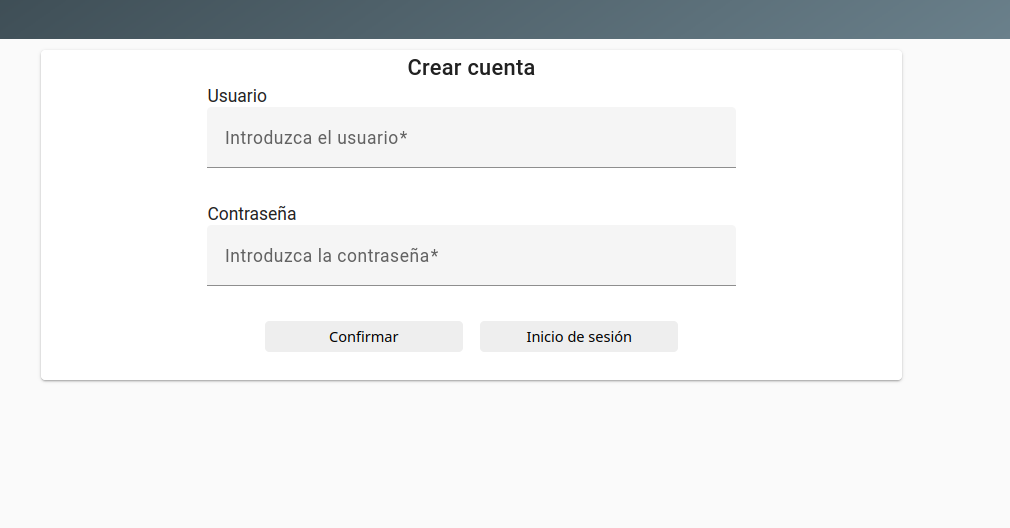
\includegraphics[width=0.7\linewidth]{img/ManualDeUsuario/crearCuenta}
	\caption{Pantalla de creación de cuenta.}
	\label{fig:crearcuenta}
\end{figure}


\subsubsection{Inicio de sesión}
Introducir el usuario y la contraseña en sus respectivas entradas de texto y pulsar el botón de confirmar, lo que llevara al usuario a la pantalla de selección de ejercicios. La pantalla de inicio de sesión se puede ver en la figura \ref{fig:iniciodesesion}. 

\begin{figure}
	\centering
	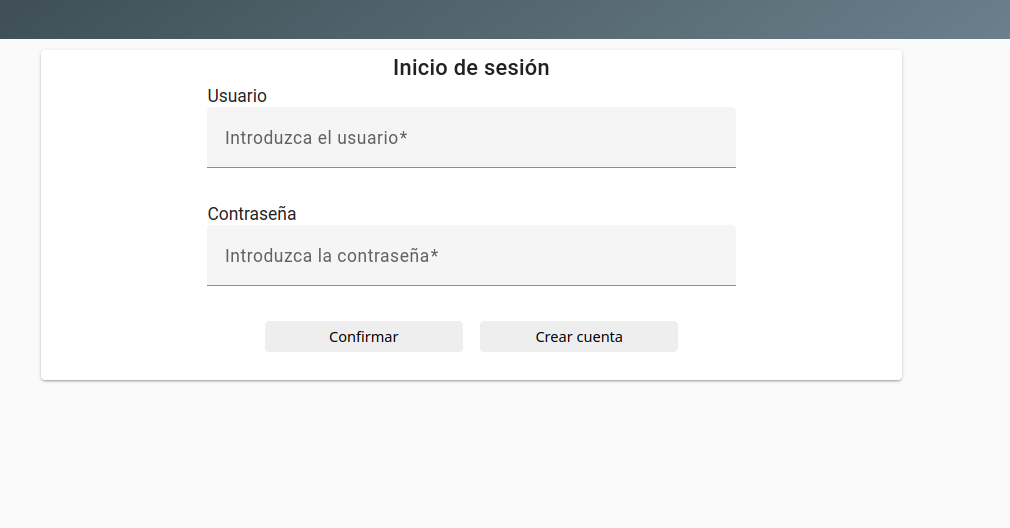
\includegraphics[width=0.7\linewidth]{img/ManualDeUsuario/inicioDeSesion}
	\caption{Pantalla de inicio de sesión.}
	\label{fig:iniciodesesion}
\end{figure}


\subsubsection{Comparación de ejercicio} 
Ir a la pagina \textit{Ejercicios} mediante el menú y seleccionar un ejercicio de la lista pulsando su nombre. Esta pagina se puede ver en la figura \ref{fig:selectordeejercicio}.

\begin{figure}
	\centering
	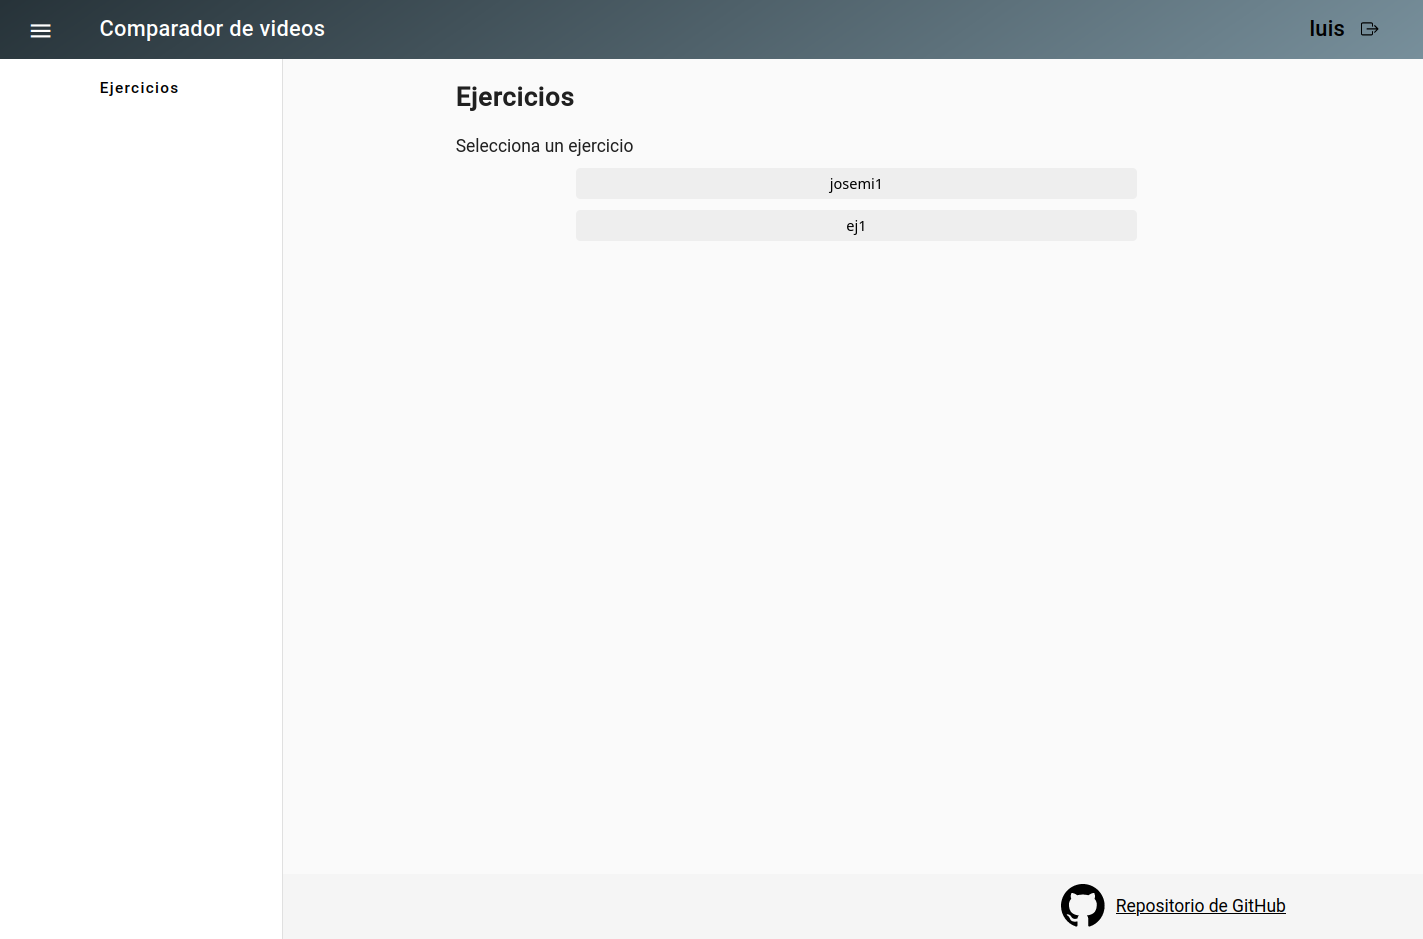
\includegraphics[width=0.7\linewidth]{img/ManualDeUsuario/selectorDeEjercicio}
	\caption{Selector de ejercicios}
	\label{fig:selectordeejercicio}
\end{figure}


Añadir un fichero y pulsar el botón de enviar. Esperar a que termine la comparación de vídeos y lleguen los resultados.

\begin{figure}
	\centering
	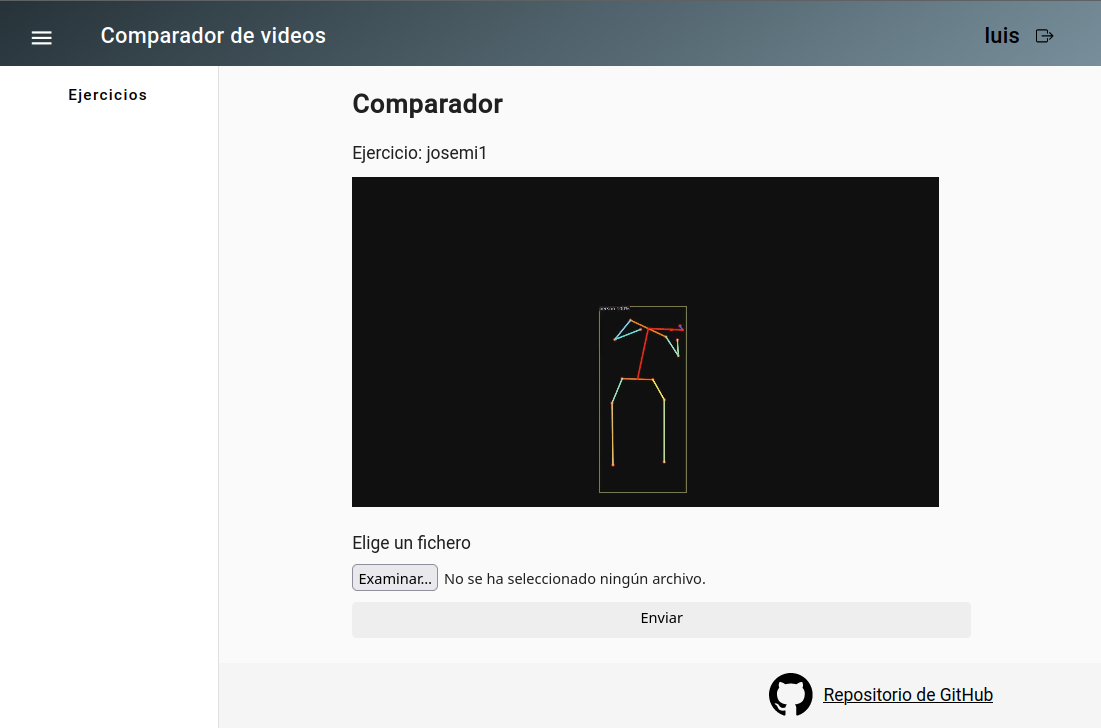
\includegraphics[width=0.7\linewidth]{img/ManualDeUsuario/comparador}
	\caption{Vista del comparador de vídeos.}
	\label{fig:comparador}
\end{figure}
Esperar a que se comparé el vídeo y llegue la puntuación, como se puede ver en la figura \ref{fig:puntuacion}.
\begin{figure}
	\centering
	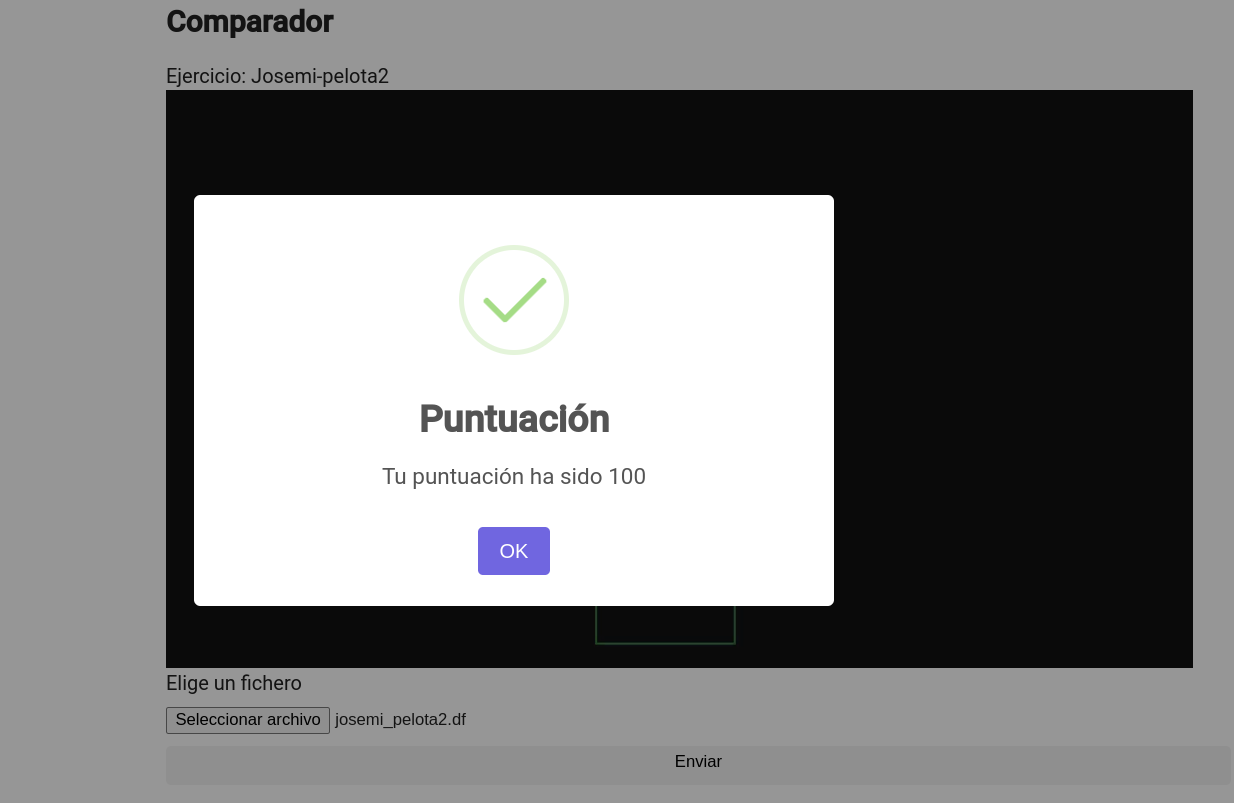
\includegraphics[width=0.7\linewidth]{img/ManualDeUsuario/puntuacion}
	\caption{Puntuación del ejercicio.}
	\label{fig:puntuacion}
\end{figure}

\subsection{Terapeuta}
El terapeuta podrá crear y borrar nuevos ejercicios para que los pacientes puedan comparar sus ejercicios con los que suba el terapeuta.La cuenta del terapeuta se crea por defecto, en el \textit{.env} se encuentran el usuario y la contraseña del mismo en las variables \texttt{FIRST\_SUPERUSER} y \texttt{FIRST\_SUPERUSER\_PASSWORD}.
\subsubsection{Creación de ejercicio}
\begin{enumerate}
	\item Escribir el nombre del ejercicio.
	\item Añadir el fichero de datos del ejercicio.
	\item Añadir un vídeo.
	\item Seleccionar los ángulos y coordenadas.
	\item Pulsar el botón de confirmar.
\end{enumerate}

\begin{figure}
	\centering
	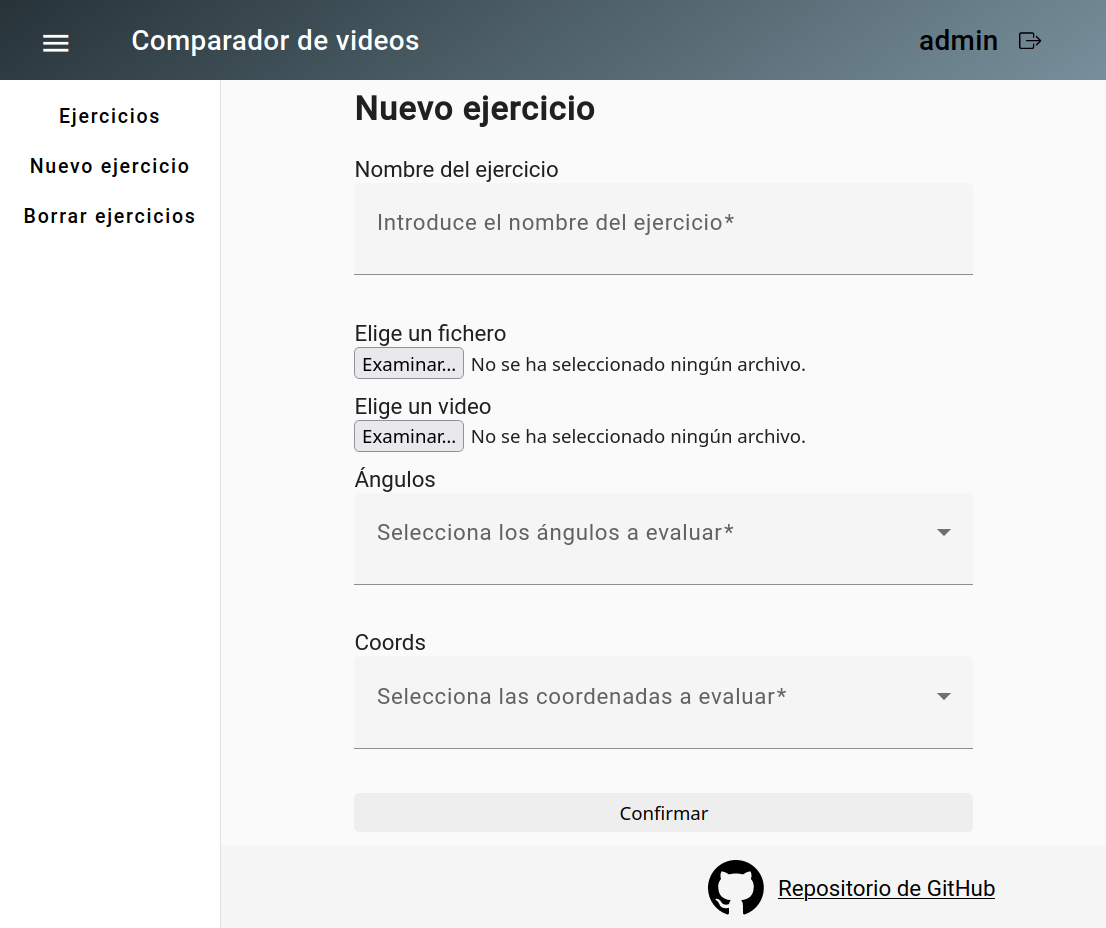
\includegraphics[width=0.7\linewidth]{img/ManualDeUsuario/nuevoEjercicio}
	\caption{Vista de nuevo ejercicio.}
	\label{fig:nuevoejercicio}
\end{figure}


\subsubsection{Borrar ejercicio}
Para eliminar el ejercicio bastará con pulsar el botón de borrar que se encuentra al lado del nombre del ejercicio como se puede ver en la pantalla \ref{fig:borrarejercicio}.
\begin{figure}
	\centering
	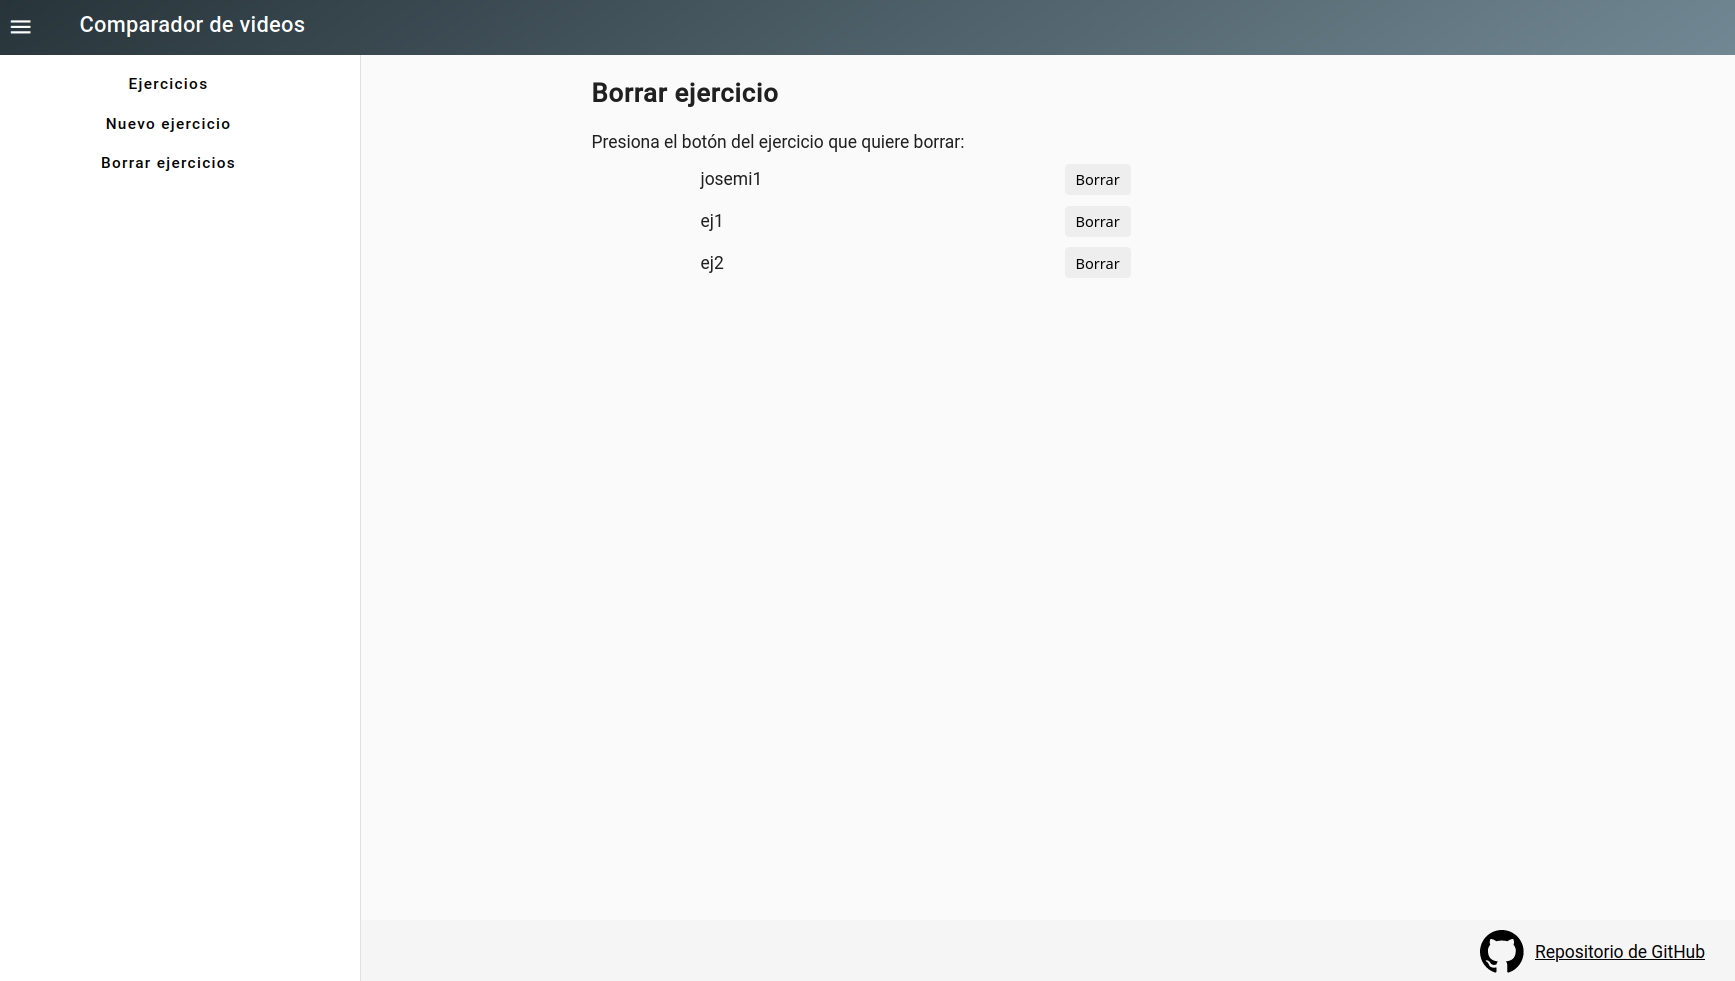
\includegraphics[width=0.7\linewidth]{img/ManualDeUsuario/borrarEjercicio}
	\caption{Pantalla para borrar ejercicios.}
	\label{fig:borrarejercicio}
\end{figure}

Una vez presionado el botón saldrá una modal en la que habrá que presionar el botón \textit{Borrar} como se puede observar en la figura \ref{fig:borrarejercicioconfirmacion}.
\begin{figure}
	\centering
	\includegraphics[width=0.7\linewidth]{img/ManualDeUsuario/borrarEjercicioConfirmación}
	\caption{Confirmación de que se desea borrar el ejercicio.}
	\label{fig:borrarejercicioconfirmacion}
\end{figure}

